\begin{frame}[fragile]{Introduction}
Neural networks have found recent success as controllers for dynamical systems

\centering
\begin{figure}
    \begin{subfigure}{0.45\textwidth}
        \centering
        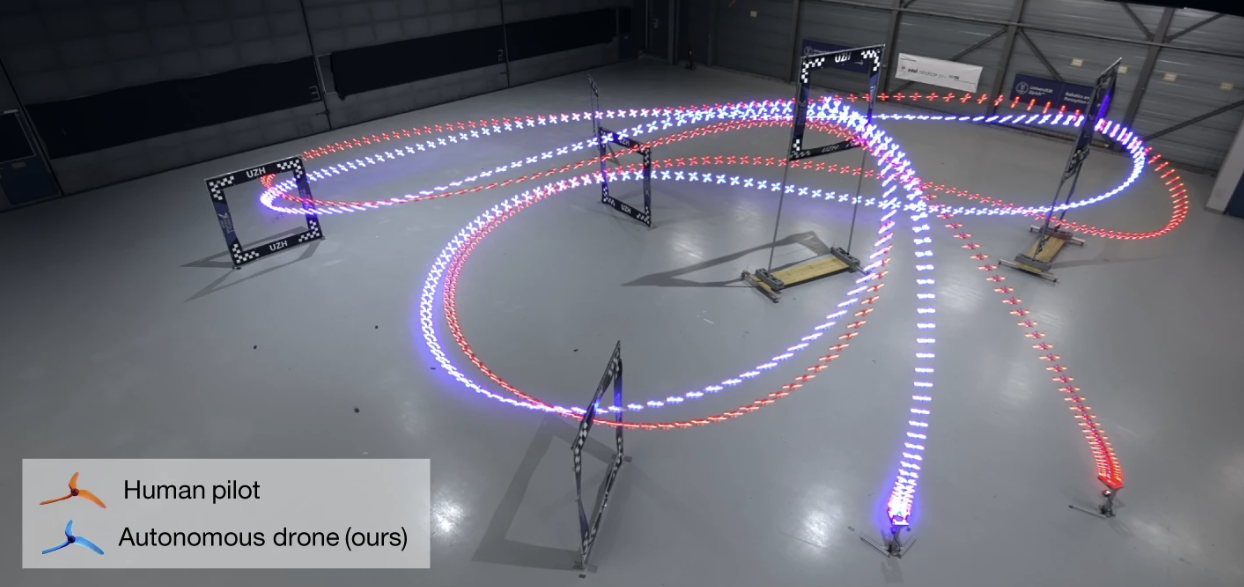
\includegraphics[width=\textwidth, height=0.4\textheight]{slides/OvertPoly/figs/droneRacing.png}
        \caption{Drone Racing \footnotemark[1]}
    \end{subfigure}
    \begin{subfigure}{0.45\textwidth}
        \centering
        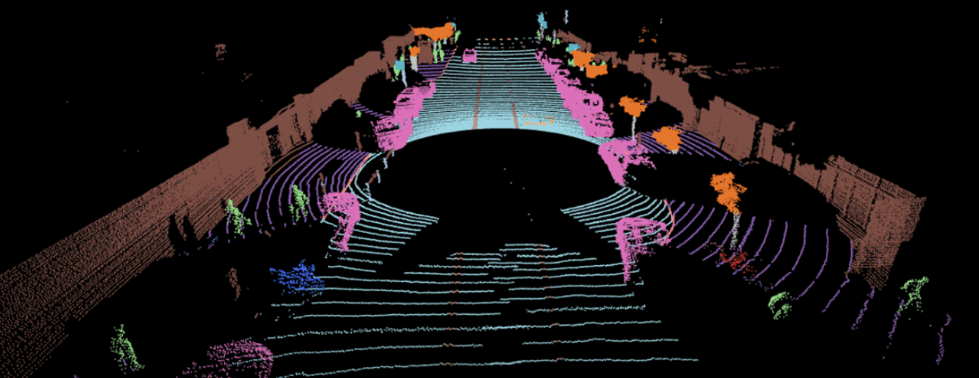
\includegraphics[width=\textwidth, height=0.4\textheight]{slides/OvertPoly/figs/waymo.png}
        \caption{Autonomous Driving \footnotemark[2]}
    \end{subfigure}
    \footnotetext[1]{Credit: \footcite{kaufmann2023champion}}
    \footnotetext[2]{Credit: \footcite{ettinger2021large}}
\end{figure}
\end{frame}

\begin{frame}[fragile]{Neural Feedback Systems}
    The resulting systems are what we call \emph{Neural Feedback Systems} (NFS)
    \begin{figure}
        \begin{center}
            \begin{tikzpicture}
                % Nodes
                \node (plant) [draw, rectangle, minimum width=1.5cm, minimum height=1cm, label=above:{Plant}] {$f(x)$};
                \node (controller) [draw, below=1.5cm of plant, rectangle, minimum width=1.5cm, minimum height=1cm, label=below:{Controller}] {$\pi(y)$};
                \node (input) [draw, left= 2cm of plant, circle]{$+$};
                \node (noise) [above=0.5cm of input]{$\epsilon$};
                \node (observer) [draw, below right=0.25cm and 1.5cm of plant, rectangle, minimum width=1.5cm, minimum height=1cm, label=right:{Sensor}] {$o(x)$};

                % Edges
                \draw[->] (noise) -- (input);
                \draw[->] (controller) -| (input)node[pos=0.3, yshift=7pt]{$u$};
                \draw[->] (input) -- (plant);
                \draw[->] (plant) -| (observer);
                \draw[->] (observer) |- (controller) node[midway, xshift=7pt, yshift=7pt]{$y$};
            \end{tikzpicture}
        \end{center}
    \end{figure}
\end{frame}

\begin{frame}[fragile]{Neural Feedback Systems}
    \begin{columns}
        \column{0.4\textwidth}
        \begin{figure}
            \resizebox{\columnwidth}{!}{
                \begin{tikzpicture}
                    % Nodes
                    \node (plant) [draw, rectangle, minimum width=1.5cm, minimum height=1cm, label=above:{Plant}] {$f(x)$};
                    \node (controller) [draw, below=1.5cm of plant, rectangle, minimum width=1.5cm, minimum height=1cm, label=below:{Controller}] {$\pi(y)$};
                    \node (input) [draw, left= 2cm of plant, circle]{$+$};
                    \node (noise) [above=0.5cm of input]{$\epsilon$};
                    \node (observer) [draw, below right=0.25cm and 1.5cm of plant, rectangle, minimum width=1.5cm, minimum height=1cm, label=right:{Sensor}] {$o(x)$};
    
                    % Edges
                    \draw[->] (noise) -- (input);
                    \draw[->] (controller) -| (input)node[pos=0.3, yshift=7pt]{$u$};
                    \draw[->] (input) -- (plant);
                    \draw[->] (plant) -| (observer);
                    \draw[->] (observer) |- (controller) node[midway, xshift=7pt, yshift=7pt]{$y$};
                \end{tikzpicture}
            }
        \end{figure}

        \column{0.6\textwidth}
        Assume $x \in \mathbb{R}^n, f(x) = [f_1(x), \ldots, f_n(x)]$, where each $f_i: \mathbb{R}^n \to \mathbb{R}$, $\epsilon \in E$, $\pi$ is a neural network

        \vspace{0.5cm}
        The system ($\mathcal{D}$) evolves such that for each $i \in [1..n]$
        \begin{align*}
            \mathit{next}^{\mathcal{D}}(x)_i = \Big\{x_i + \big(f_i(x) + \pi(o(x))_i + \epsilon\big) \cdot \delta | \epsilon \in E\Big\}
        \end{align*}

        where $\delta$ is the time step size, and $E$ the error set
    \end{columns}
\end{frame}

\begin{frame}[fragile]{Neural Feedback Systems}
    \begin{columns}
        \column{0.4\textwidth}
        \begin{figure}
            \resizebox{\columnwidth}{!}{
                \begin{tikzpicture}
                    % Nodes
                    \node (plant) [draw, rectangle, minimum width=1.5cm, minimum height=1cm, label=above:{Plant}] {$f(x)$};
                    \node (controller) [draw, below=1.5cm of plant, rectangle, minimum width=1.5cm, minimum height=1cm, label=below:{Controller}] {$\pi(y)$};
                    \node (input) [draw, left= 2cm of plant, circle]{$+$};
                    \node (noise) [above=0.5cm of input]{$\epsilon$};
                    \node (observer) [draw, below right=0.25cm and 1.5cm of plant, rectangle, minimum width=1.5cm, minimum height=1cm, label=right:{Sensor}] {$o(x)$};
    
                    % Edges
                    \draw[->] (noise) -- (input);
                    \draw[->] (controller) -| (input)node[pos=0.3, yshift=7pt]{$u$};
                    \draw[->] (input) -- (plant);
                    \draw[->] (plant) -| (observer);
                    \draw[->] (observer) |- (controller) node[midway, xshift=7pt, yshift=7pt]{$y$};
                \end{tikzpicture}
            }
        \end{figure}

        \column{0.6\textwidth}
        A NFS is the tuple
        $\langle n,I,F,E,u,\delta, T, G, A\rangle$, where 
        \begin{itemize}
            \uncover<1->{\item $n$ is the dimensionality of the system} 
            \uncover<2->{\item $I$ is the set of initial states}
            \uncover<3->{\item $F$ is the set of functions $f_i$}
            \uncover<4->{\item $E$ is the bounded error set}
            \uncover<5->{\item $u$ is the neural network controller}
            \uncover<6->{\item $\delta$ is the time step size}
            \uncover<7->{\item $T$ is the time horizon}
            \uncover<8->{\item $G$ is the set of goal states}
            \uncover<9->{\item $A$ is the set of unsafe states at each time step}
        \end{itemize}

    \end{columns}
\end{frame}

\begin{frame}[fragile]{Reach-Avoid Properties}
    \begin{columns}
        \column{0.4\textwidth}
        \begin{figure}
            \resizebox{\columnwidth}{!}{
                \begin{tikzpicture}
                    % Nodes
                    \node (plant) [draw, rectangle, minimum width=1.5cm, minimum height=1cm, label=above:{Plant}] {$f(x)$};
                    \node (controller) [draw, below=1.5cm of plant, rectangle, minimum width=1.5cm, minimum height=1cm, label=below:{Controller}] {$\pi(y)$};
                    \node (input) [draw, left= 2cm of plant, circle]{$+$};
                    \node (noise) [above=0.5cm of input]{$\epsilon$};
                    \node (observer) [draw, below right=0.25cm and 1.5cm of plant, rectangle, minimum width=1.5cm, minimum height=1cm, label=right:{Sensor}] {$o(x)$};
    
                    % Edges
                    \draw[->] (noise) -- (input);
                    \draw[->] (controller) -| (input)node[pos=0.3, yshift=7pt]{$u$};
                    \draw[->] (input) -- (plant);
                    \draw[->] (plant) -| (observer);
                    \draw[->] (observer) |- (controller) node[midway, xshift=7pt, yshift=7pt]{$y$};
                \end{tikzpicture}
            }
        \end{figure}

        \column{0.6\textwidth}
        A \emph{trajectory} $\tau^{\mathcal{D}}(\mathcal{X}_0)$ is a sequence of states ($\mathcal{X}_0, \mathcal{X}_1, \ldots, \mathcal{X}_T$), where $\mathcal{X}_0 \subseteq I$, and for each $t \in [1..T]$, $\mathcal{X}_{t} = \mathit{next}^{\mathcal{D}}(\mathcal{X}_{t-1})$
        
        \vspace{0.5cm}

        A system ($\mathcal{D}$) is \emph{safe} if for all trajectories $\tau^{\mathcal{D}}(\mathcal{X}_0)$,
        \begin{align}
            &\forall x_0 \in I\,.\exists t \in [0..T]\,.\, \tau^{\mathcal{D}}(\{x_0\})_t \subseteq G, \\
            &\forall t \in [0..T], \tau^{\mathcal{D}}(I)_t \cap A(t) = \emptyset
        \end{align}
    \end{columns}
\end{frame}









